\documentclass{article}
\usepackage[margin=1in, top = .8in, left=.8in]{geometry}
\usepackage{comment}
\usepackage{amsmath, amssymb}
\usepackage{framed}
\usepackage{enumerate}
\usepackage{comment}
\usepackage{tikz,pgfplots}
\usepgfplotslibrary{fillbetween}
\pgfplotsset{compat=1.15}
\usepackage[hyphens]{url}
\everymath{}

\begin{document}

\begin{center}
    \large \textbf{Homework 5}
\end{center}
    %\item[\textbf{Week 5}]
                \begin{enumerate}

    \item Evaluate the following definite integrals. The answer should be a number. If you cannot give an exact value, then give its value to within exactly four decimal points. 
    \begin{enumerate}
        \item $ \int_{-1}^{2} \frac{2}{5}z^9-{1}{4}z^3 + 3z + 1 \, dz$
        \item $ \int_1^9 \frac{\sqrt{t}-1}{t^{\frac{3}{2}}}\,dt$
        \item $ \int_0^1 p(\sqrt[3]{p}+\sqrt[4]{p})\,dp$
        \item $ \int_{0}^{2} \left| 2x-1
        \right|\,dx$
        \item $ \int_0^1 (b^2+2)^4\,db$
    \end{enumerate}

    \item The graph below shows a function $f(x) = cx(x-b)^2$. Find the value of $c$ so that the shaded blue area is equal to 1. Note that choosing the values of the parameters so that the area under the curve is 1 means that we can use this function, restricted to the appropriate domain, as a probability density function. After finding the value of $c$, use it to find the probability that a random variable with this density function lies between 0 and $ \frac{b}{2}$. What do you notice about your answer?
    \begin{center}
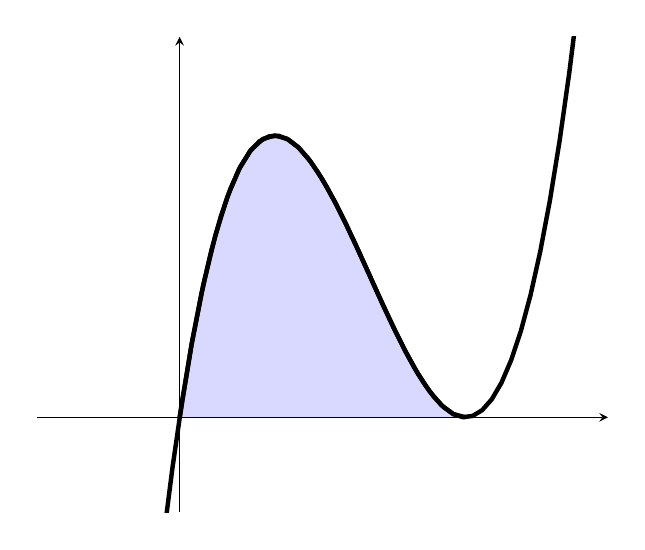
\begin{tikzpicture}
\begin{axis}[
   	xmin=-.5, xmax=1.5,
	ymin=-0.5, ymax=2,
%	xtick={2,4,6,8,10},  
%	ytick={2,4,6,8,10,12},
    yticklabels={,,},
    xticklabels={,,},
	major tick length={0},
	line width=1pt,
 	axis lines=center, height=3 in,
	]
    \addplot [ultra thick, samples=60,domain=-.5:1.5] {10*x*(x-1)^2};
    \addplot [name path = f,ultra thick, domain=0:1] {10*x*(x-1)^2};
       \path[name path=axis] (axis cs:0,0) -- (axis cs:1,0);
    \addplot [
        thick,
        color=blue,
        fill=blue, 
        fill opacity=0.15
    ]
    fill between[
        of=f and axis
    ];
\end{axis}
\end{tikzpicture}
\end{center}

                    \item Given $F'(x)=f(x)$, evaluate $ \int x^3f(2x^4)\ dx$. You may need to use $F(x)$ and/or $f(x)$ in your answer.
                    \item If $ \int_a^b f(x)\,dx = c$, what does 
                    $ \int_{a+k}^{b+k} f(x-k)\,dx$ equal? 
                    \item If $ \int_a^b f(x)\,dx = c$, what does 
                    $ \int_{a/k}^{b/k} f(kx)\,dx$ equal?
                    \item Evaluate the definite integral 
                    $ \int_{1}^{e} \frac{(\ln{x})^2}{x}\,dx$.
                    \item Evaluate $ \int x\ln(x)\ dx$.  Because $\int \ln(x)\ dx$ is not obvious, the best choice to apply integration by parts is with $f(x)=\ln(x)$ and $g'(x)=x$.
                    \item Given $F'(x)=f(x)$ and $G'(x)=F(x)$, evaluate $ \int_a^b xf(x)\ dx$, using the information on the following table. \\
                        \begin{center}
                        \begin{tabular}{|c|c|c|c|}
                        \hline
                        $x$ & $f(x)$ & $F(x)$ & $G(x)$ \\
                        \hline
                        $a$ & $2$ & $4$ & $10$ \\
                        \hline
                        $b$ & $-1$ & $5$ & $-11$ \\
                        \hline 
                        \end{tabular}
                        \end{center}
                        \medskip
                        
                    \item Find the value of $c$ so that the function 
                    $ \frac{c\ln{x}}{x^2}$ defines a probability density function on the interval $[1,2]$. (Hint: What must the area under the curve be?)
                    
                    \item Confirm using technology that $ \int_{-1}^{1} \frac{1}{\sqrt{2\pi}} \exp\left(-\frac{x^2}{2}\right)\,dx \approx 0.6827$. This shows that the probability that a standard normal random variable lies between $-1$ and $1$ is $68.27\%$. Now, without using technology, find the following integrals. Show your work.
                    $$ \int_{-1}^{1} \frac{1}{\sqrt{2\pi}}x \exp\left(-\frac{x^2}{2}\right)\,dx$$.
                    $$ \int_{-1}^{1} \frac{1}{\sqrt{2\pi}}x^2 \exp\left(-\frac{x^2}{2}\right)\,dx$$.
                    \item Use the results of the previous exercise to evaluate $ \int_{\mu-\sigma}^{\mu+\sigma} \frac{1}{\sqrt{2\pi \sigma^2}}x \exp\left(-\frac{(x-\mu)^2}{2\sigma^2}\right)\,dx$. 
                    
                    \emph{Hint}: You may consider first apply the formulas derived in exercises 4 and 5 above (in that order) to rewrite the integral.

                \end{enumerate}


\end{document}
